\documentclass{article}
\usepackage[utf8]{inputenc}
\usepackage[T1]{fontenc}
\usepackage{amssymb,amsmath,amsthm,graphicx,tikz,caption,subcaption,pgfplots,hyperref,float}
\pgfplotsset{compat=1.18}
\usepackage[dvipsnames]{xcolor}
\usepackage{tikz-3dplot}
\usetikzlibrary{patterns}
\usetikzlibrary{graphs, arrows.meta}
\usetikzlibrary{colorbrewer}
\pgfplotscreateplotcyclelist{exotic}{
    teal,every mark/.append style={fill=teal!80!black},mark=*\\
    orange,every mark/.append style={fill=orange!80!black},mark=square*\\
    cyan!60!black,every mark/.append style={fill=cyan!80!black},mark=triangle*\\
    red!70!white,mark=star\\
    lime!80!black,every mark/.append style={fill=lime},mark=diamond*\\
    red,densely dashed,every mark/.append style={solid,fill=red!80!black},mark=*\\
    yellow!60!black,densely dashed,
        every mark/.append style={solid,fill=yellow!80!black},mark=square*\\
    black,every mark/.append style={solid,fill=gray},mark=otimes*\\
    blue,densely dashed,mark=star,every mark/.append style=solid\\
    red,densely dashed,every mark/.append style={solid,fill=red!80!black},mark=diamond*\\
}

\begin{document}

	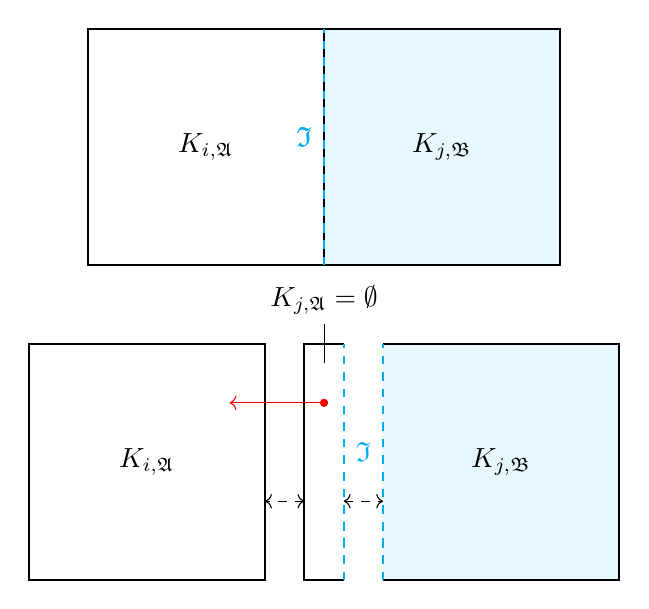
\begin{tikzpicture}
  % Background mesh cells

    \pgfmathsetmacro{\xSize}{3}
    \pgfmathsetmacro{\ySize}{3}
	\pgfmathsetmacro{\offSet}{1}


	  % Interface

	  % upper picture
	  \fill[cyan!10] (2*\xSize, \ySize) -- (\xSize, \ySize) -- (\xSize,0) -- (2*\xSize,0) -- cycle;
	  \draw[thick] (0,0) rectangle (\xSize,\ySize);
	  \draw[thick] (\xSize,0) rectangle (2*\xSize,\ySize);
	  \draw[domain=0:3, samples=100, cyan, thick, dashed] plot ({\xSize}, {(\x)});


	  \node[text=cyan] at (\xSize*11/12,\ySize*6.5/12) {$\mathfrak{I}$};

	  % Labels
	  \node at (\xSize/2,\ySize/2) {$K_{i,\mathfrak{A}}$};
	  \node at (3/2*\xSize,\ySize/2) {$K_{j,\mathfrak{B}}$};

	% lower picture
	\fill[cyan!10] (2*\xSize+0.75, -\offSet) -- (\xSize+0.75, -\offSet) -- (\xSize+0.75,-\ySize-\offSet) -- (2*\xSize+0.75,-\ySize-\offSet) -- cycle;
	\draw[thick] (0-0.75,-\ySize-\offSet) rectangle (\xSize-0.75,-\offSet);
	\draw[thick] (\xSize+0.25,-\offSet) -- (\xSize-0.25,-\offSet) -- (\xSize-0.25,-\ySize-\offSet) -- (\xSize+0.25,-\offSet-\ySize);
	\draw[thick] (\xSize+0.75,-\offSet) -- (2*\xSize+0.75,-\offSet) -- (2*\xSize+0.75,-\ySize-\offSet) -- (\xSize+0.75,-\ySize-\offSet) ;
	\draw[domain=0:3, samples=100, cyan, thick, dashed] plot ({\xSize+0.25}, {(\x-\ySize-\offSet)});
	\draw[domain=0:3, samples=100, cyan, thick, dashed] plot ({\xSize+0.75}, {(\x-\ySize-\offSet)});

	\node[text=cyan] at (\xSize*11/12,\ySize*6.5/12) {$\mathfrak{I}$};

	% Labels
	\node at (0.75,\ySize/2-\ySize-\offSet) {$K_{i,\mathfrak{A}}$};
	\draw (\xSize,-5/4*\offSet) -- (\xSize,-3*\offSet/4) node[left,above=0pt] {$K_{j,\mathfrak{A}} = \emptyset$};
	\node at (5.25,\ySize/2-\ySize-\offSet) {$K_{j,\mathfrak{B}}$};
 	\node[text=cyan] at (\xSize*13/12+0.25,\ySize*6.5/12-\ySize-\offSet) {$\mathfrak{I}$};

 	\draw [dashed, <->] (\xSize*11/12,-\ySize) --  (\xSize*9/12,-\ySize);
 	\draw [dashed, <->] (\xSize*13/12,-\ySize) --  (\xSize*15/12,-\ySize) ;

	 \fill [red] (\xSize,-7/4*\offSet) circle (1.5pt);
	 \draw [red,->]  (\xSize,-7*\offSet/4) -- ++(-\xSize*0.4,0);









  % Plot border
\end{tikzpicture}

\end{document}